\section{Preliminary Definitions}
\label{sec:background}

\subsection{Domain-Specific Languages}

As aforementioned, a DSL is a set of language constructs each of which represents certain abstraction in a particular domain. In the general case, a DSL offers an editor that provides the capabilities needed to write programs (textually or graphically) by using the language constructs. Once a the program is written, it can be used as part of the implementation artifacts of a system under construction. 

Like general purpose languages (GPLs), DSLs are specified in terms of three interdependent dimensions: abstract syntax, concrete syntax, and semantics \cite{Harel:2004b}. The \textit{abstract syntax} refers to the structure of the DSL and specifies each language construct in terms of its name and the relationships it has with other language constructs of the DSL. The \textit{concrete syntax} refers to the association of the language constructs to the set of symbols (either graphical or textual) offered by the editor. Finally, the \textit{semantics} of a DSL refers to the meaning of the language constructs and it is expressed through static constraints and dynamic behavior. The static constraints usually correspond to the type system of the DSL. In turn, the dynamic behavior defines the manner in which language constructs are manipulated at runtime, typically through the definition of an interpreter or compiler.

\textbf{Scope:} In this paper we are interested on DSLs which abstract syntax is specified by means of metamodels and semantics is specified operationally as a set  methods (a.k.a, \textit{domain-specific actions} \cite{Combemale:2013}) on the metaclasses of the metamodel. In other words, each language construct is specified as a metaclass and the relationship between language constructs are specified as references between metaclasses. In turn, each metaclass contains a set of methods that correspond to the behavior in runtime. The concrete syntax is out of the scope of this paper. 

%A DSL is specified in terms of its abstract syntax, concrete syntax and semantics. There is a mapping between the concrete syntax and the semantics. Then, a DSL specification can be defined as triple $<AS, CS, Sem>$.

\subsection{On the notions of \textit{commonalities} and \textit{potential reuse} in DSLs}

Due to the complexity of current systems, there is a large amount of concerns to deal with. In addition, by definition the domain of a DSL is scoped to a specific aspect of a system. As a result, there is a proliferation of many DSLs in the literature \cite{Mernik:2005b}. Although many of those existing DSLs are completely different and tackle independent domains; there are related DSLs with overlapping domains. That is, they share certain language constructs. When two DSLs share language constructs, we say that there is \textbf{potential reuse} since the specification of those shared constructs can be reused in the two DSLs \cite[p. 60-61]{voelter:2013}.

\begin{figure}
\centering
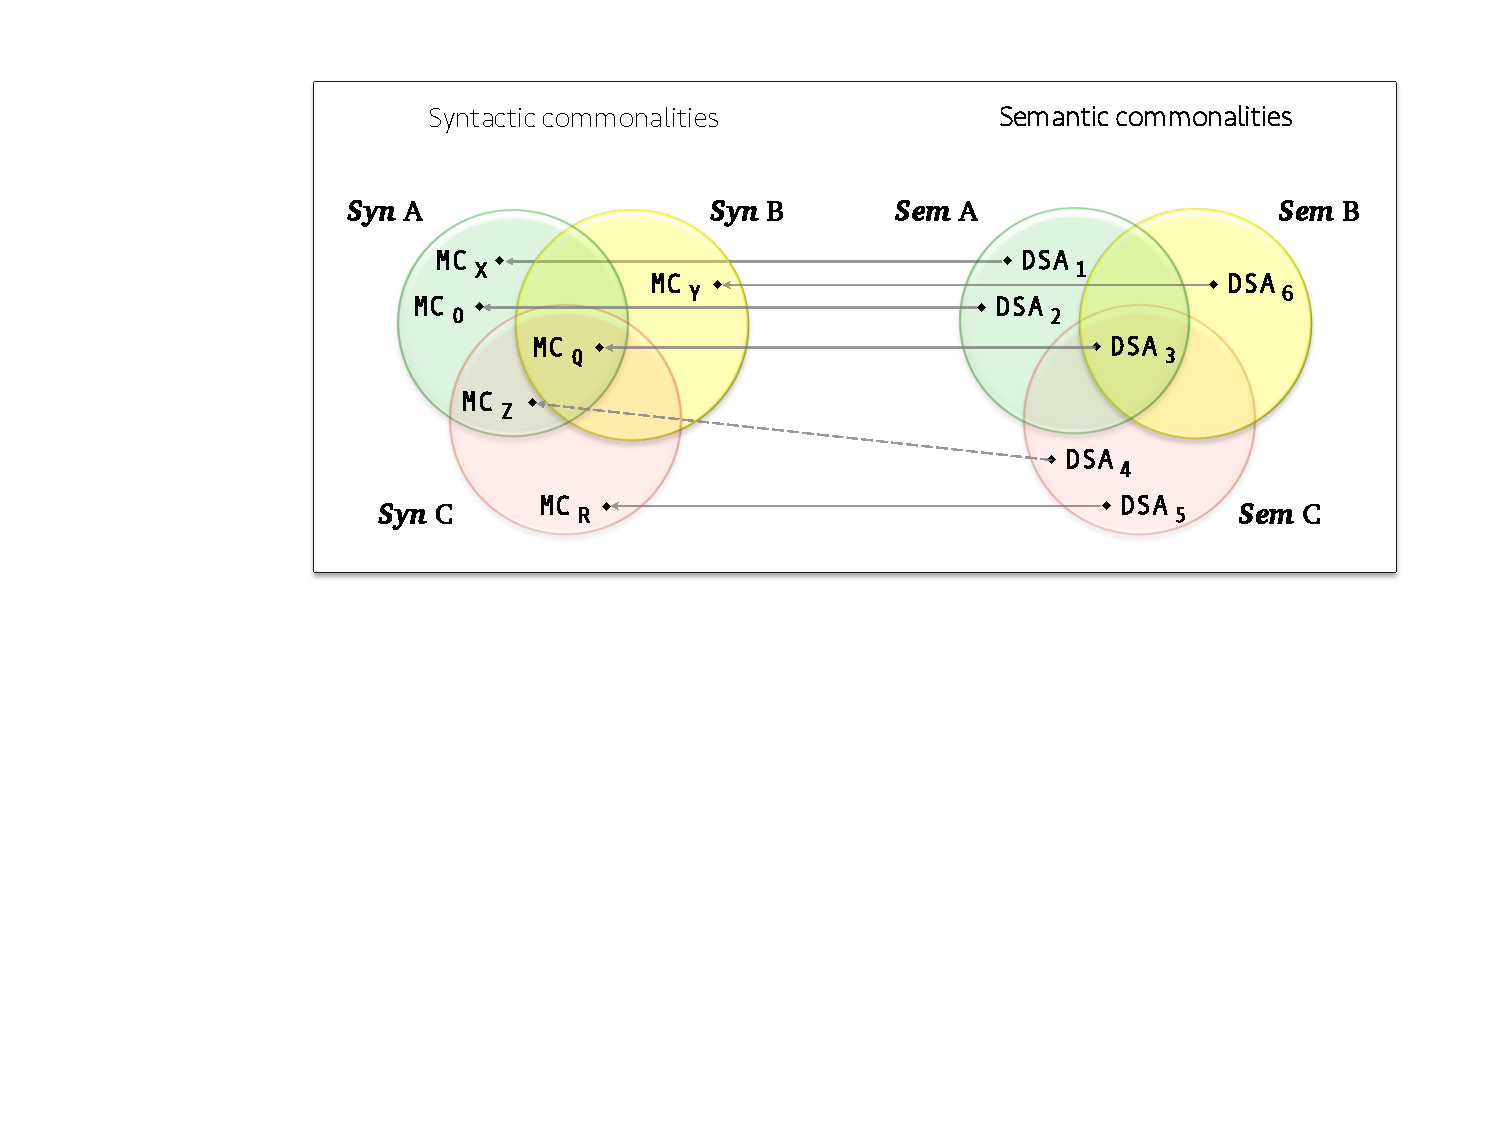
\includegraphics[width=1\linewidth]{images/domains-fig.pdf}
\caption{Commonalities between domains and potential reuse}
\label{fig:domains}
\end{figure}

Figure \ref{fig:domains} illustrates the situation explained above. At the left of the figure there are two DSLs that are totally independent. That means that they do not share any of their language constructs, and consequently, there is not potential reuse between them. Differently, the two DSLs shown at the right of the figure have overlapping domains. That means that there are a subset of language that are \large\textbf{``equal'' }\normalsize in both DSLs. Note that if two language constructs are the same, we can assume that their specifications are equal and can be reused instead of being replicated.


%Moreover, there are set of DSLs for which the domains can be hierarchically organized \cite[p. 60-61]{voelter:2013}.

\subsection{Equivalence between language constructs}

So far, we have based the notion of potential reuse in DSLs on the commonalities existing in a set of DSLs. Nevertheless, this assumption supposes that we are able to compare two language constructs in order to know if they are equivalent. So, now we need to define this \textit{equivalence} relationship. In particular, the comparison of two language constructs relies on two dimensions: (1) comparison of the meta-classes in the abstract syntax; and (2) comparison of the domain-specific actions in the semantics.

\vspace{-2mm}
\subsubsection{Comparing meta-classes.} The name of a metaclass usually corresponds to a word that evokes the domain concept the metaclass represents. Thus, intuitively one can think that a first approach to compare meta-classes is by comparing their name. As we will see later in this paper, this approach results quite useful and it is quite probable that, we can find potential reuse.

Unfortunately, comparison of metaclasses by using only their names might have some problems. There are cases in which two meta-classes with the same name are not exactly the same since they do not represent the same domain concept or because there are domains that use similar vocabulary. In such cases, an approach that certainly helps is to compare meta-classes not only by their names but also by their attributes and references. Although this second approach might be too restrictive, it implies that the specification of the two meta-classes are exactly the same so potential reuse is guaranteed. 

In the approach present in this paper, we provide support for the two comparison approaches explained above. However, additional comparison operators such as the surveyed in \cite{Lafi:2011} can be easily incorporated.

\vspace{-2mm}
\subsubsection{Comparing domain-specific actions.} Like methods in Java, domain-specific actions have a signature where the contract is specified (i.e., return type, visibility, parameters, name, and so on), and a body where the behavior is actually implemented. In that sense, the comparison of two domain-specific actions can be performed by checking if their signatures are equal. This approach is practical and also reflects potential reuse; one might think that the probability that two domain-specific actions with the same signatures are the same is elevated. 

However, as the reader might imagine, there are cases in which signatures comparison is not enough. Two domain-specific actions defined in different DSLs can perform different computations even if they have the same signatures. As a result, a second approach relies in the comparison of the bodies of the domain-specific actions. Note that such comparison can be arbitrary complex task. Indeed, if we try to compare  the behavior of the actions we will have to deal with the semantic equivalence problem that, indeed, is known as be undecidable \cite{Lucanu:2013}. In this case, we a conservative approach is to compare onlythe structure (abstract syntax tree) body of the domain-specific action.

In our approach we support both comparison operators: the one based on the signature and the one based on the signature and the body. To the later, we use the API for java code comparison proposed in \cite{Biegel:2010}. 

\vspace{-2mm}
\subsubsection{Semantical variability.} A necessary condition to decide whether two language constructs are equivalent is that both, the metaclass and the associated domain-specific actions are equivalent. This condition guarantees that the specification is the same not only at the level of the abstract syntax but also at the level of the semantics. However, there is a phenomenon in the literature that corresponds to semantical variability \cite{Cengarle:2009}. There is semantical variability when there there are two constructs that have the same abstract syntax (i.e., their metaclasses are equal) but that differ in the domain-specific actions. This case is of interest for us because even in the presence of semantical variability we can have some potential reuse. If the metaclasses of two constructs are the same we can reuse them even if their domain-specific actions are different. 
